\documentclass[10pt,a4paper]{article}
\usepackage[utf8]{inputenc}
\usepackage[english]{babel}
\usepackage{amsmath}
\usepackage{amsfonts}
\usepackage{amssymb}
\usepackage{graphicx}
\usepackage{indentfirst}
\usepackage{fancyvrb}
\usepackage{microtype}
\usepackage{subfigure}
\usepackage{booktabs}
\usepackage[hidelinks]{hyperref}
\author{Giuseppe L'Erario}
\date{}

\title{Support Vector Machine}
 
\begin{document}
\maketitle
\section*{Introduction}
\emph{Support vector machines} are supervised learning models used mainly for classification purpose.

In \emph{Support vector machines} objective is to maximize the distance (the \textbf{margin}) between the decision boundary (the \textbf{hyperplanes}) and the training samples closer to it. These samples are the \textbf{support vectors}.

One can find the good balance between bias an overfitting tuning the margins.


\section{Linear Support Vector Machine}
\emph{Linear} SVMs are used for classification of linearly separable datasets. However, with the introduction of a \emph{slack} variable we can relax the linear constraints in order to work on nonlinearly separable data.

The coefficient of this variable is the \textbf{C} parameter, that rules the penalty for a misclassification. Large values of \textbf{C} correspond to large penalties and vice versa. To tune the \textbf{C} parameter is necessary to control the  width of the margin and find the compromise between bias and overfitting.

In this homework we work on the famous \emph{Iris dataset}. Only the first two features of the dataset are imported. Then, the dataset is divided in a train, a validation and a test set. The first two sets are used to train the classifier and tune the parameters, while the test set is used to measure the performance\footnote{Use the test set to tune the parameters in order to increase the accuracy transforms it in a train set at all.}. 

In fig.\ref{linear_svm} it is clear how the decision boundaries vary with the \textbf{C} parameter. To a low value of \textbf{C} (fig.\ref{C_0001}) corresponds high bias. Increasing \textbf{C}, and therefore the penalty for a misclassification, the boundaries become more precise.

\begin{figure}[h]
	\centering
	\subfigure[C=0.001\label{C_0001}]{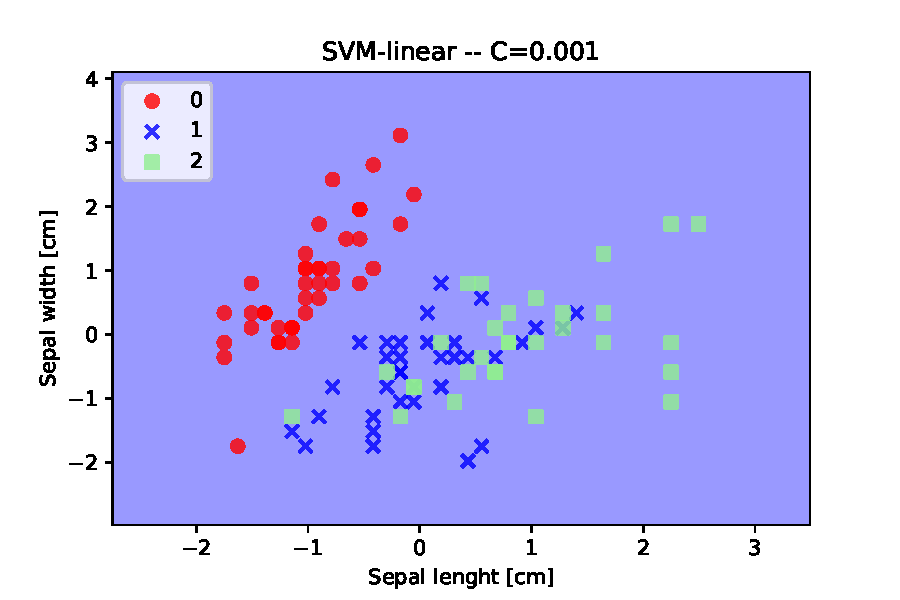
\includegraphics[width=0.4\linewidth]{../Images/lin_C0001.pdf}}\qquad\qquad
	\subfigure[C=0.01\label{C_001}]{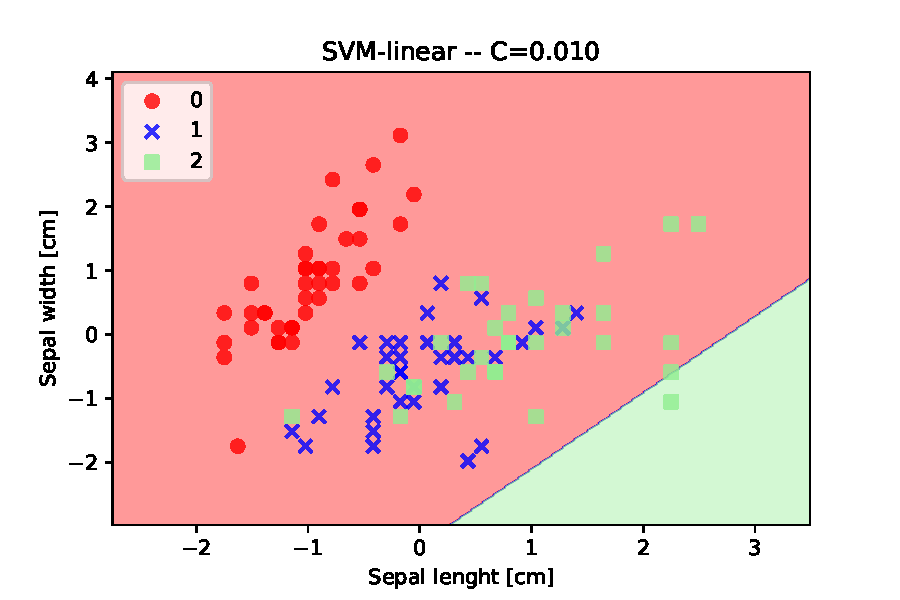
\includegraphics[width=0.4\linewidth]{../Images/lin_C001.pdf}}
\end{figure}
\begin{figure}
	\centering
	%\addtocounter{figure}%	\ContinuedFloat
	\subfigure[C=0.1\label{C_01}]{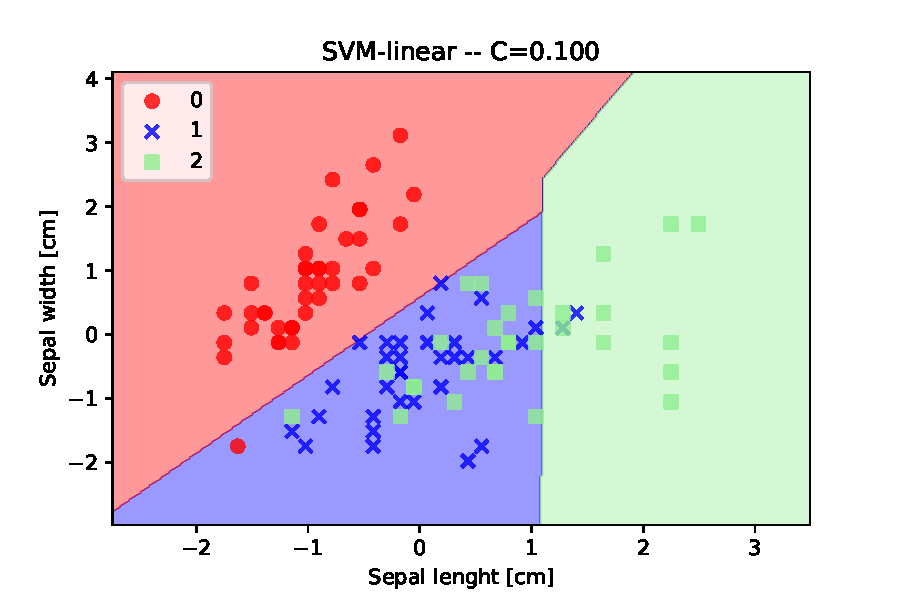
\includegraphics[width=0.4\linewidth]{../Images/lin_C01.pdf}}\qquad\qquad
	\subfigure[C=1\label{C_1}]{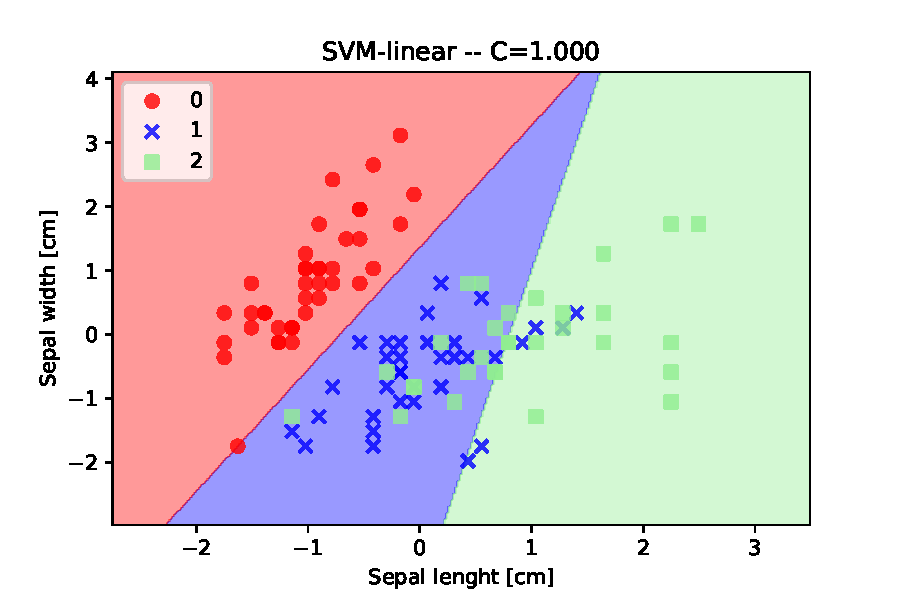
\includegraphics[width=0.4\linewidth]{../Images/lin_C1.pdf}}
	\subfigure[C=10\label{C_10}]{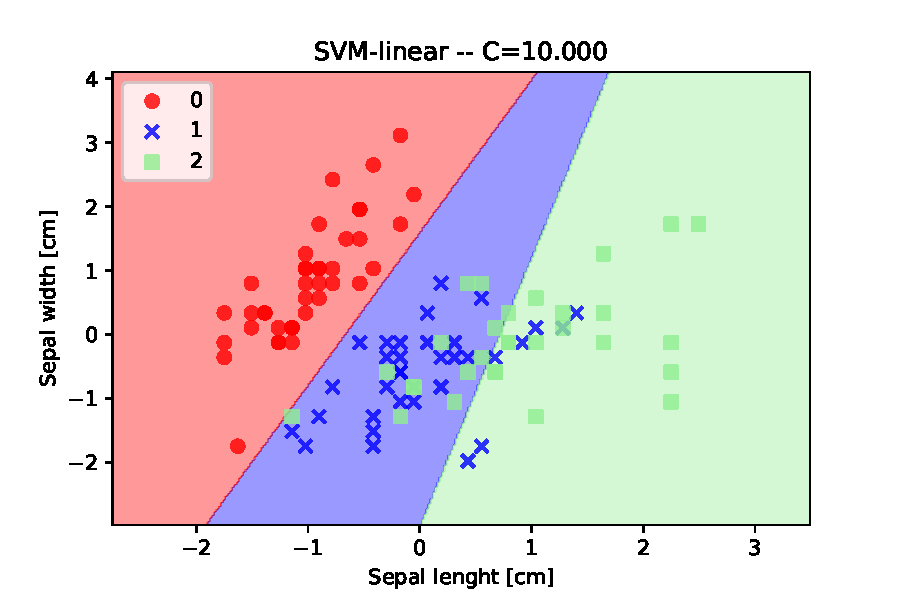
\includegraphics[width=0.4\linewidth]{../Images/lin_C10.pdf}}\qquad\qquad
	\subfigure[C=100\label{C_100}]{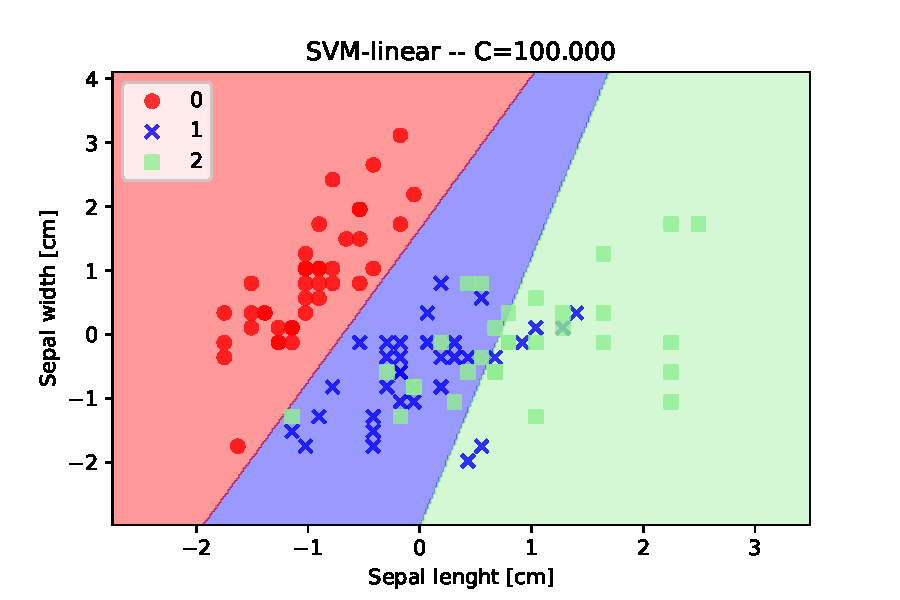
\includegraphics[width=0.4\linewidth]{../Images/lin_C100.pdf}}
	\subfigure[C=1000\label{C_1000}]{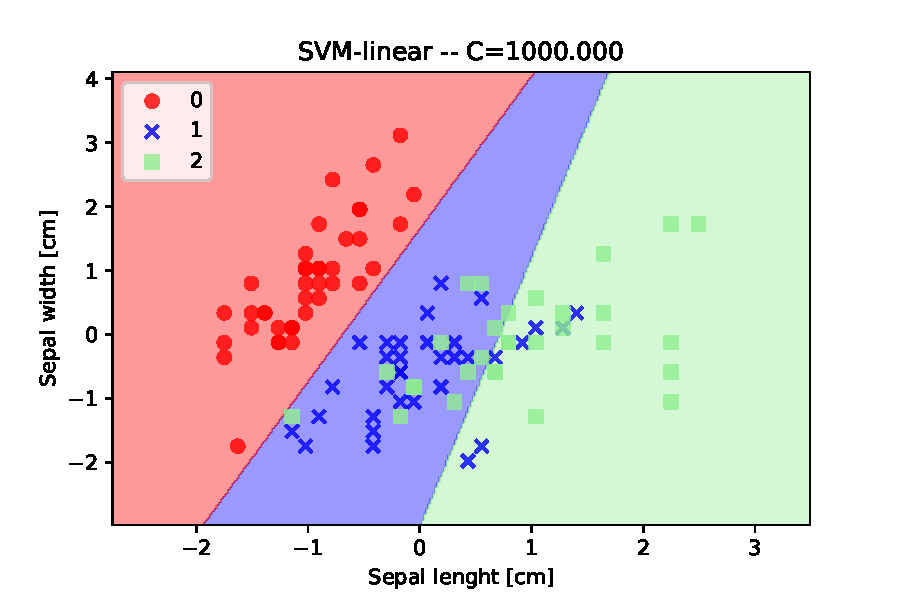
\includegraphics[width=0.4\linewidth]{../Images/lin_C1000.pdf}}
	\caption{Linear SVM.\label{linear_svm}}
\end{figure}

The fig.\ref{fig:c_accuracy} shows how the accuracy varies with the \textbf{C} parameter.

\begin{figure}
	\centering
	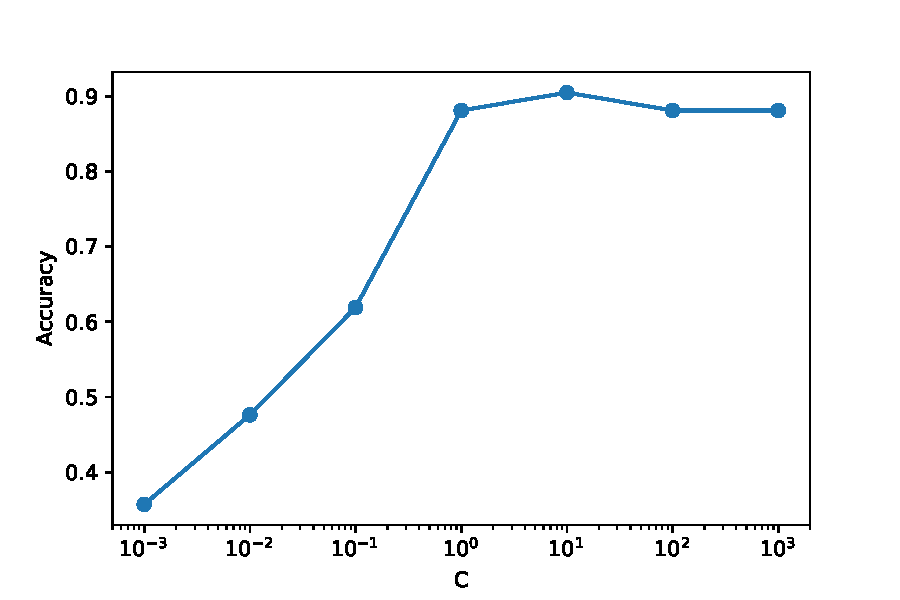
\includegraphics[width=0.7\linewidth]{../Images/c_accuracy.pdf}
	\caption{Accuracy - \textbf{C} parameter.}
	\label{fig:c_accuracy}
\end{figure}

The best score obtained on validation set is evaluated on the test set, in fig.\ref{fig:lin_C10_best}, achieving an accuracy of 71.1\%.

\begin{figure}
\centering
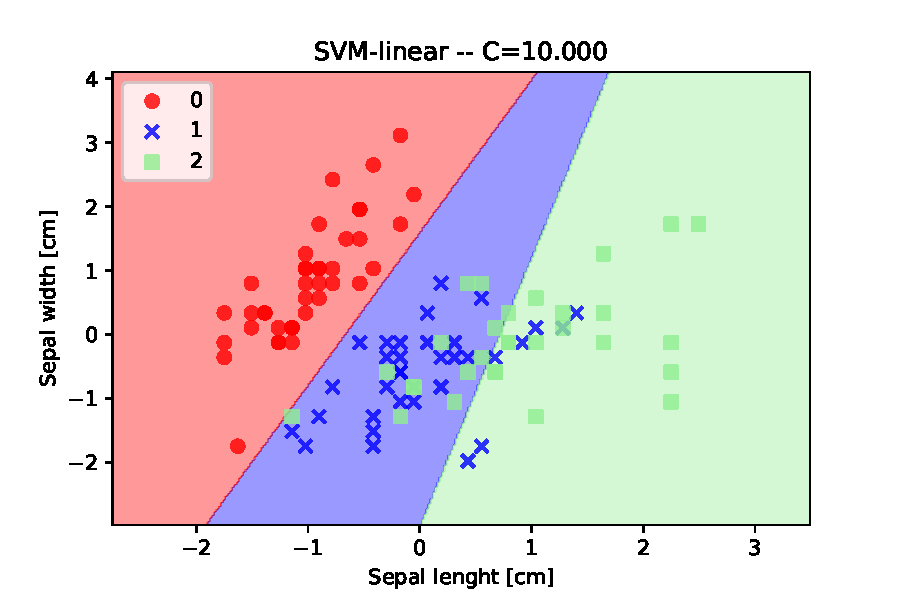
\includegraphics[width=0.7\linewidth]{../Images/lin_C10_best.pdf}
\caption{Evaluation on Test set.}
\label{fig:lin_C10_best}
\end{figure}


\section{RBF Vector Machine}
To solve a nonlinear problem we transform the training data onto a higher dimensional space with a mapping function and train a linear classifier. Then the same mapping function is used to transform the data to classify.

This approach, based on the dot product between features, is computationally expensive. Here come out the benefit of a kernel function $k(x_i \cdot x_j)=f(x_i) \cdot f(x_j)$ that avoids the use of dot product.

One of the most used kernel function is the \textbf{Radial Basis function kernel}:
\begin{equation}
	k(x_i \cdot x_j) = e^{-\gamma\|x_i - x_j\|^2}
\end{equation}
where $\gamma$ is a parameter to optimize.

\subsubsection*{Fixed $\mathbf{\gamma}$}
The behaviour on varying of \textbf{C} is similar to linear SVM. The difference is in the curved decision boundaries.
\begin{figure}[!h]
	\centering
	\subfigure[C=0.001\label{rbgC_0001}]{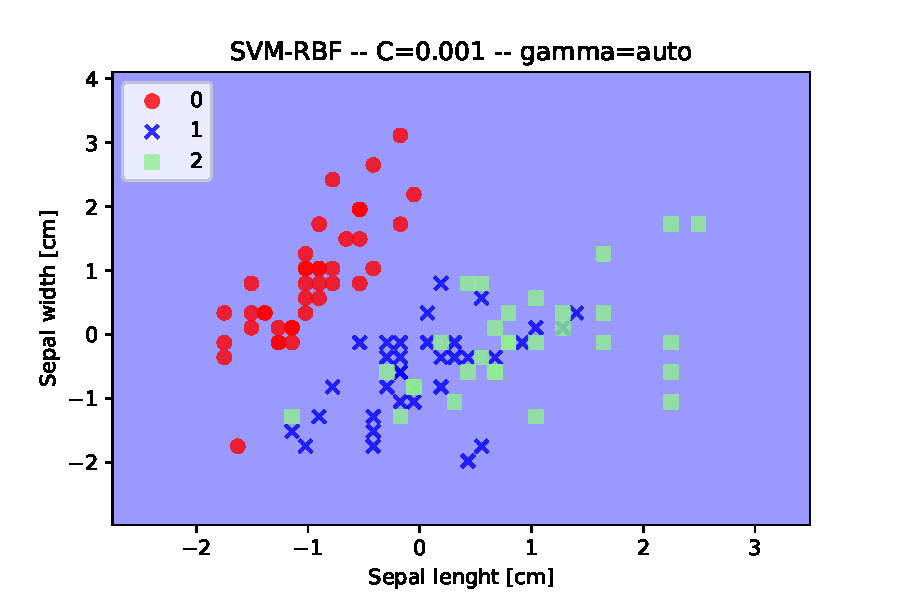
\includegraphics[width=0.4\linewidth]{../Images/rbf_C0001.pdf}}\qquad\qquad
	\subfigure[C=0.01\label{rbfC_001}]{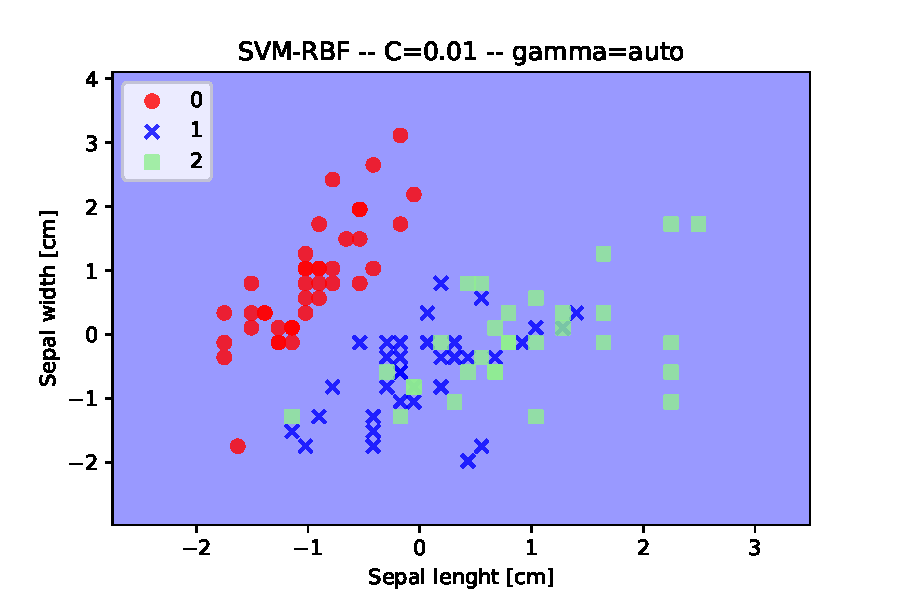
\includegraphics[width=0.4\linewidth]{../Images/rbf_C001.pdf}}
	\subfigure[C=0.1\label{rbfC_01}]{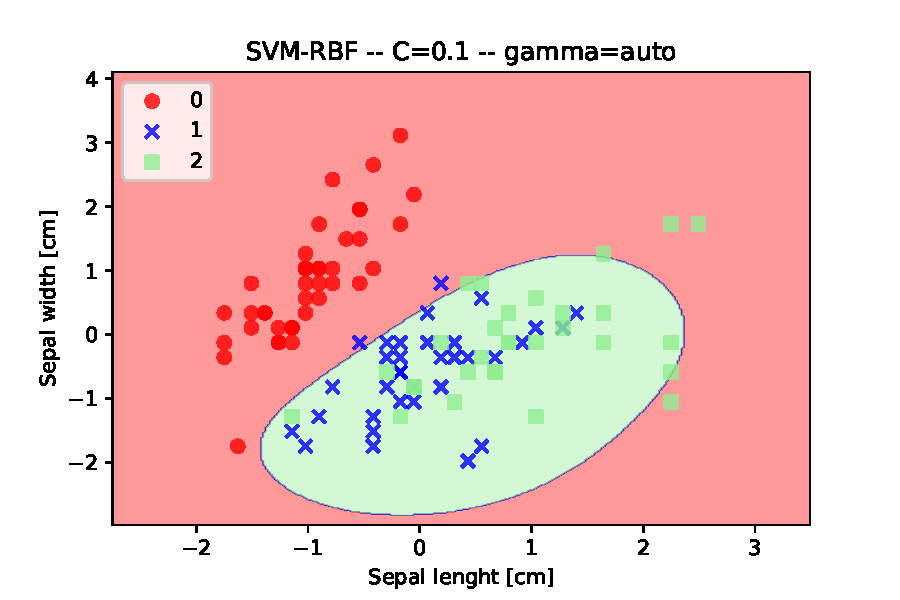
\includegraphics[width=0.4\linewidth]{../Images/rbf_C01.pdf}}\qquad\qquad
	\subfigure[C=1\label{rbfC_1}]{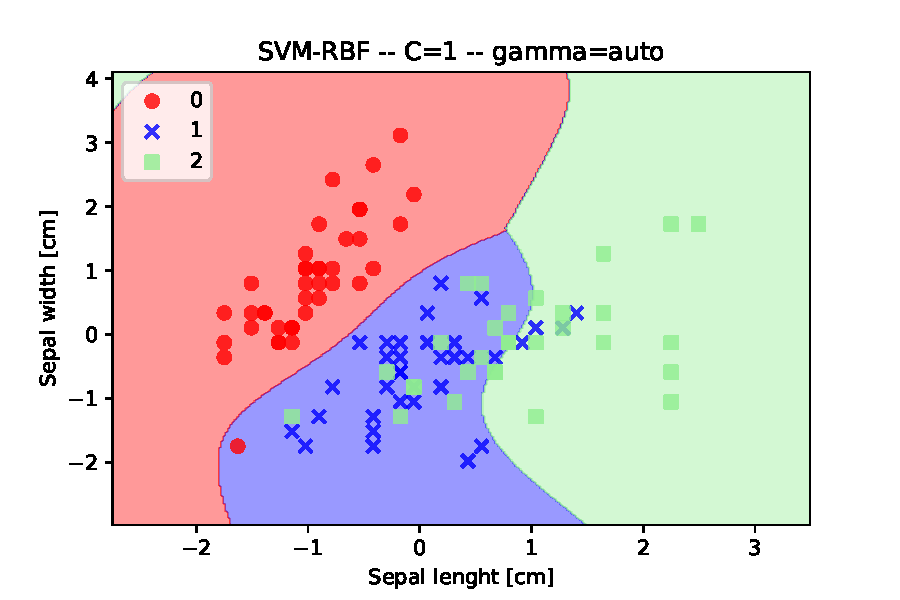
\includegraphics[width=0.4\linewidth]{../Images/rbf_C1.pdf}}
	\subfigure[C=10\label{rbfC_10}]{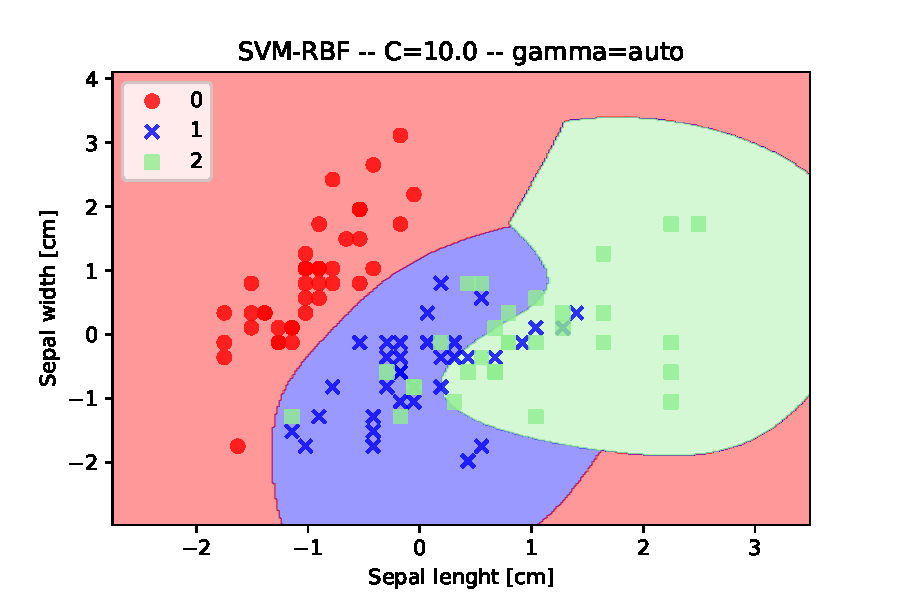
\includegraphics[width=0.4\linewidth]{../Images/rbf_C10.pdf}}\qquad\qquad
	\subfigure[C=100\label{rbfC_100}]{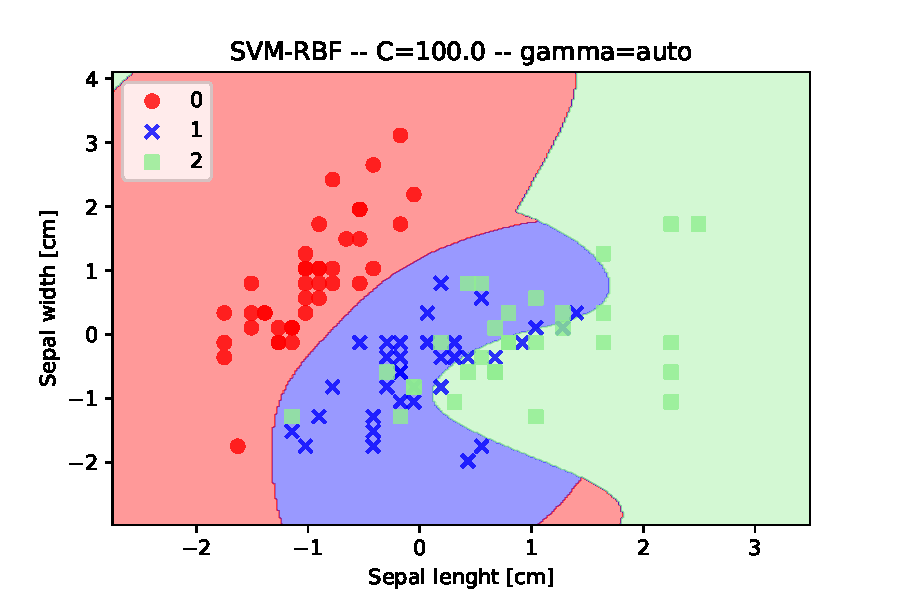
\includegraphics[width=0.4\linewidth]{../Images/rbf_C100.pdf}}
	\subfigure[C=1000\label{rbfC_1000}]{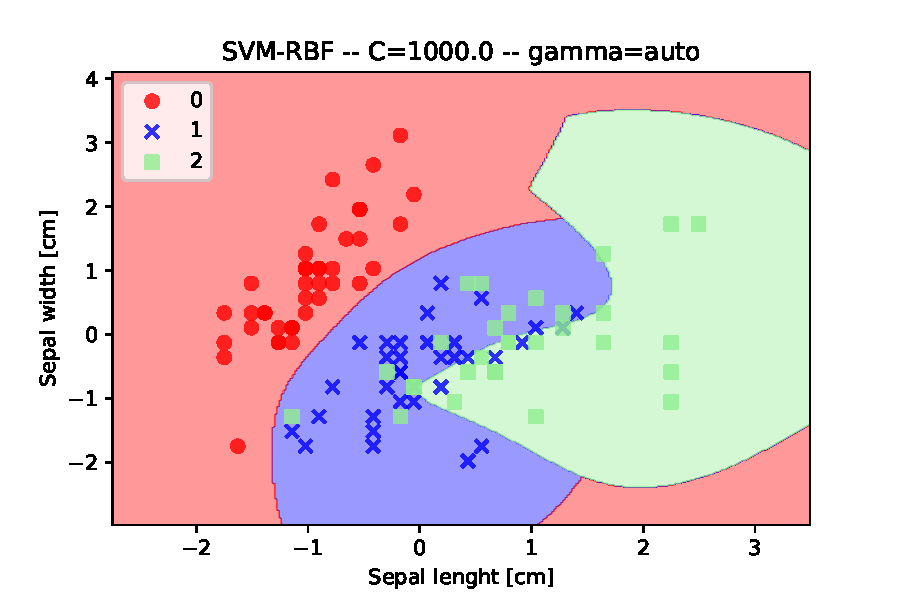
\includegraphics[width=0.4\linewidth]{../Images/rbf_C1000.pdf}}
	\caption{RBF SVM with $\gamma=auto$.\label{rbf_svm_c}}
\end{figure}
	 
	
The best score obtained on validation set is evaluated on the test set, in fig.\ref{fig:rbf_C1_best}, achieving an accuracy of 71.4\%.

\begin{figure}[t]
\centering
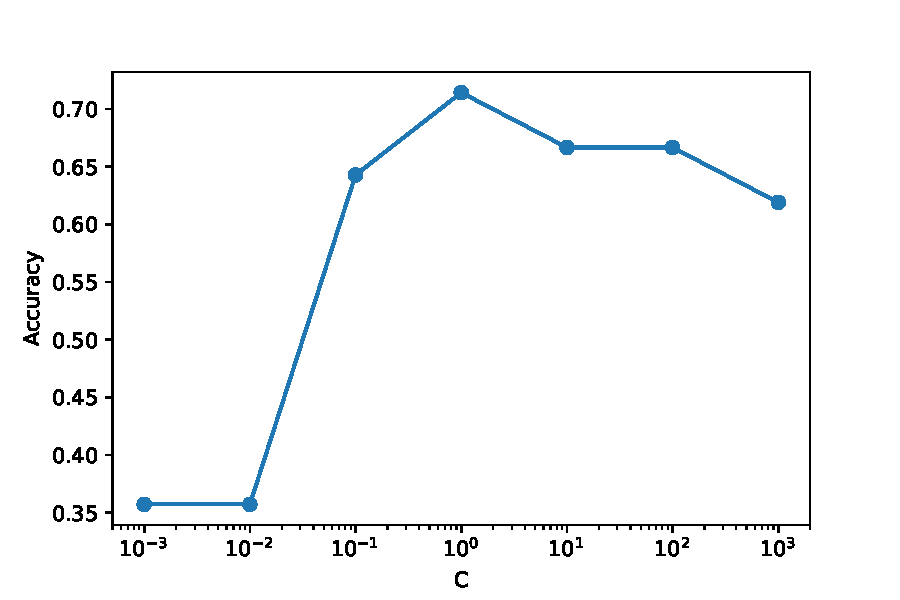
\includegraphics[width=0.7\linewidth]{../Images/c_accuracy_rbf_c.pdf}
\caption{Accuracy - \textbf{C} parameter.}
\label{fig:c_accuracy_rbf_c}
\end{figure}

\begin{figure}
\centering
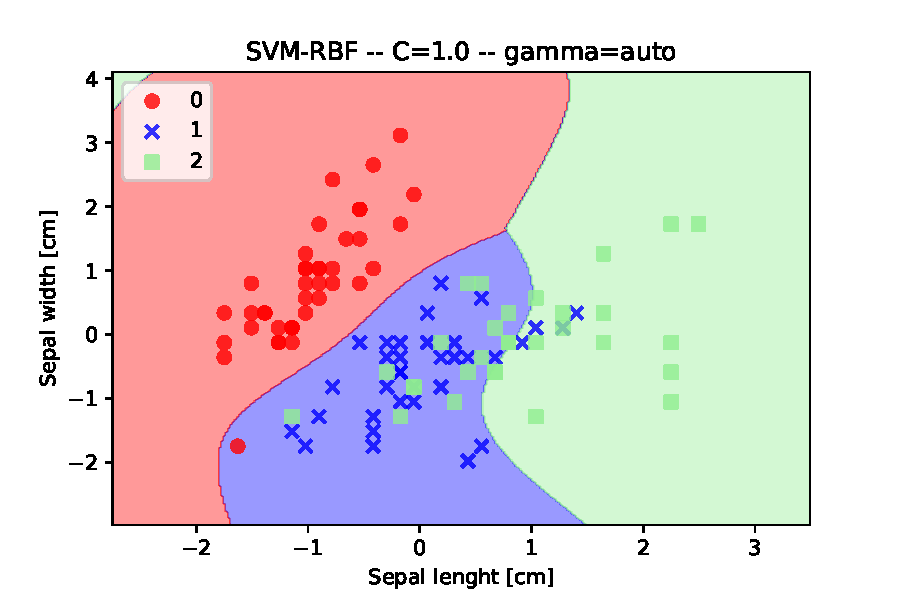
\includegraphics[width=0.7\linewidth]{../Images/rbf_C1_best.pdf}
\caption{Evaluation on Test set.}
\label{fig:rbf_C1_best}
\end{figure}

\subsubsection*{Grid search}
The $\gamma$ parameter is not anymore fixed. To find the best combination we use a grid search.

\begin{table}[!h]
	\centering
\begin{tabular}{c | c c c c c c}
	\toprule
	\textbf{C}/$\gamma$ & $0.0001$ & $0.001$ & $0.1$ & $10$ & $1000$ & $100000$ \\
	\midrule 
	$0.001$ & $21.42$ & $21.42$ & $21.42$ & $21.42$ & $21.42$ & $21.42$ \\
	$0.01$  & $21.42$ & $21.42$ & $21.42$ & $21.42$ & $21.42$ & $21.42$ \\
	$0.1$  & $21.42$ & $21.42$ & $23.82$ & $21.42$ & $21.42$ & $21.42$ \\
	1 & $21.42$ & $21.42$ & $69.04$ & $57.14$ & $21.42$ & $21.42$ \\
	10 & $21.42$ & $35.71$ & $69.04$ & $52.38$ & $21.42$ & $21.42$ \\
	100 & $21.42$ & $69.04$ & \textbf{76.19} & $52.38$ & $21.42$ & $21.42$ \\
	1000 & $38.09$ & $69.04$ & $71.42$ & $52.38$ & $21.42$ & $21.42$ \\
	\bottomrule
\end{tabular}
\caption{Grid Search}\label{Grid_search}
\end{table}

The result of the grid search, in tab.\ref{Grid_search}, is that the best parameters are $C=100$ and $\gamma=0.1$, as we can see in fig.\ref{fig:validation_accuracy}.

\begin{figure}
\centering
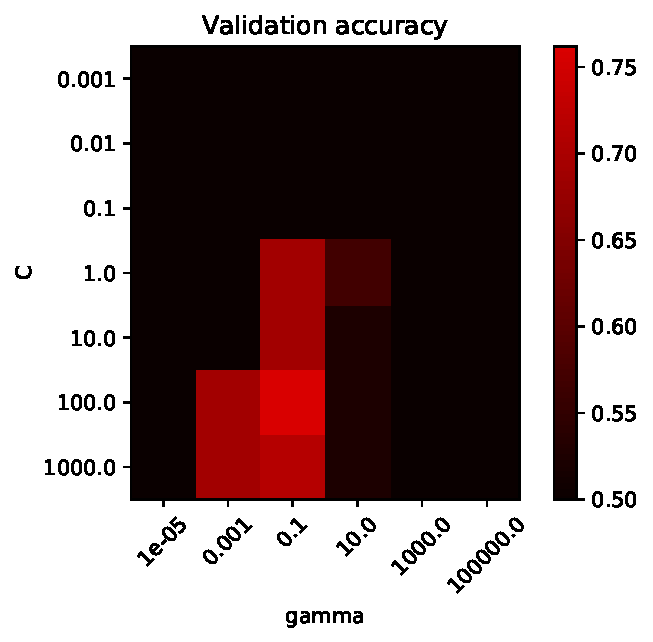
\includegraphics[width=0.7\linewidth]{../Images/validation_accuracy}
\caption{Heatmap for \textbf{C} and $\gamma$.}
\label{fig:validation_accuracy}
\end{figure}

These parameters, evaluated on the test set (see fig.\ref{fig:rbf_C100G01_best}), give an accuracy of 67\%, worse then the accuracy on validation set.

\begin{figure}[!]
\centering
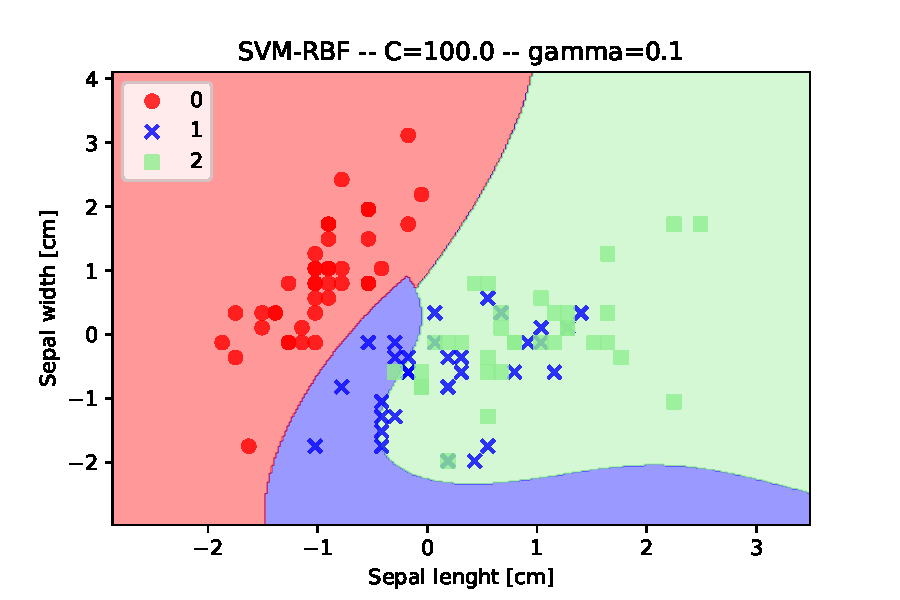
\includegraphics[width=0.7\linewidth]{../Images/rbf_C100G01_best}
\caption{Evaluation on Test set}
\label{fig:rbf_C100G01_best}
\end{figure}

\section{K-fold validation}

In \textbf{k-fold validation} the training set is splitted in \emph{k} folds, where 1 fold is used for validation and the others for training. This procedure is repeated \emph{k} times (choosing every time one different fold for validation) and in order to obtain \emph{k} evaluation. Then is computed the average accuracy for the model. 

The aim is to find a less sensitive estimation to the partitioning of the set.    

\begin{table}[h]
	\centering
	\begin{tabular}{c | c c c c c c}
		\toprule
		\textbf{C}/$\gamma$ & $0.0001$ & $0.001$ & $0.1$ & $10$ & $1000$ & $100000$ \\
		\midrule 
		$0.001$ & $38.09$ & $38.09$ & $38.09$ & $38.09$ & $38.09$ & $38.09$ \\
		$0.01$  & $38.09$ & $38.09$ & $38.09$ & $38.09$ & $38.09$ & $38.09$ \\
		$0.1$  & $38.09$ & $38.09$ & $40.00$ & $38.09$ & $38.09$ & $38.09$ \\
		1 & $38.09$ & $38.09$ & $78.09$ & ${81.90}$ & $67.61$ & $67.61$ \\
		10 & $38.09$ & $53.33$ & 78.09  & $80.00$ & $67.61$ & $61.61$ \\
		100 & $38.09$ & $78.09$ & $\mathbf{83.10}$ & $80.00$ & $67.61$ & $67.61$ \\
		1000 & $54.28$ & $80.95$ & $80.95$ & $80.00$ & $67.61$ & $67.61$ \\
		\bottomrule
	\end{tabular}
	\caption{Grid Search with k-fold validation}\label{Grid_search_k}
\end{table}

From tab.\ref{Grid_search_k} and fig.\ref{fig:validation_accuracy_k} we can see that the best accuracy is placed in correspondence of $C=100$ and $\gamma=0.1$, the same parameters found without k-fold validation, but with a different accuracy (83.10\% vs 76.19\%).

\begin{figure}[h]
\centering
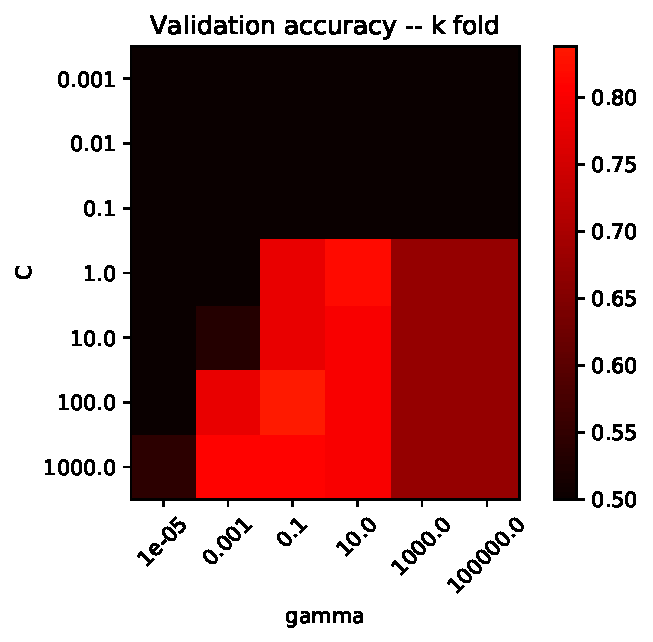
\includegraphics[width=0.7\linewidth]{../Images/validation_accuracy_k}
\caption{Heatmap for \textbf{C} and $\gamma$}
\label{fig:validation_accuracy_k}
\end{figure}


It might sound like that the k-fold validation is useless, but it is not. Infact running several simulation the performances measured are less oscillating than the ones without k-fold validation. This means that the choice of the parameters is more robust.

\begin{figure}
\centering
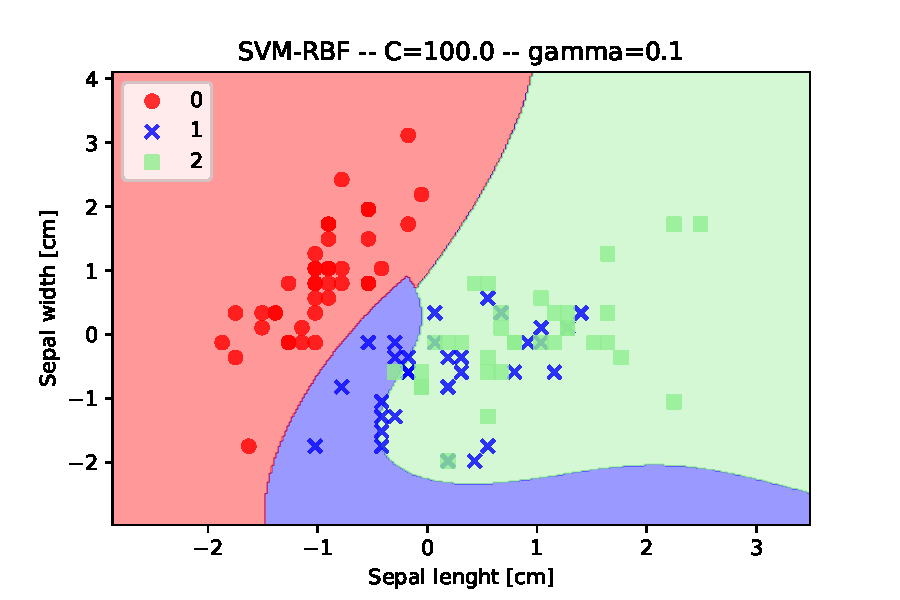
\includegraphics[width=0.7\linewidth]{../Images/rbf_C100G01_best_k}
\caption{Evaluation on test set}
\label{fig:rbf_C100G01_best_k}
\end{figure}

The evaluation on the test set, in fig.\ref{fig:rbf_C100G01_best_k} gives an accuracy of 67\%.


\end{document}